

如果初始架构开始看起来像意大利面,或者只是想阻止架构成为意大利面,将组件分层结构化可能会有所帮助。还记得“模型-视图-控制器”吗?或者类似的模式,例如“模型-视图-视图模型”或“实体-控制-边界”?这些都是分层架构的示例(如果各层在物理上彼此分离,也称为N层架构)。可以在层中构造代码,创建微服务层,或将此模式应用到可以带来利益的其他领域。引入层的主要原因是,其提供了抽象和关注点分离,还可以降低复杂性,同时改进解决方案的模块化、可重用性和可维护性。

一个真实的案例是在自动驾驶中,各个层可以用于分层决策:最底层处理汽车的传感器,然后另一层提取传感器数据的单个特征。在这一层之上,可能还有一层来确保所有特征都能是安全行为。当更换另一款汽车的时,只需要更换最底层的传感器即可。

分层架构通常很容易实现,因为大多数开发者对层的概念相当熟悉——只需要开发几个层,然后像下图那样堆叠就好:

\begin{center}
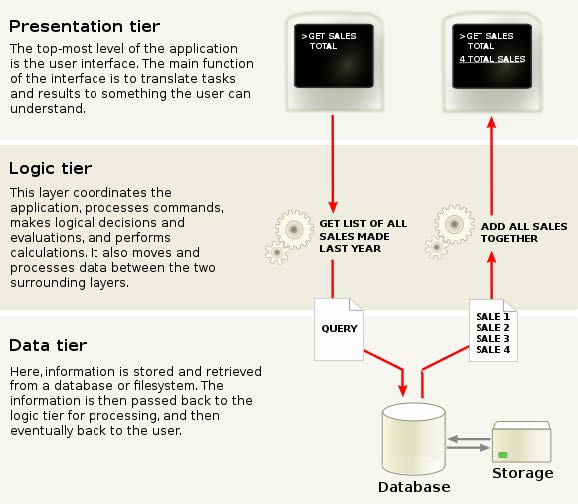
\includegraphics[width=0.9\textwidth]{content/1/chapter2/images/4.jpg}\\
图2.4 -表示层中使用文本接口的三层架构示例
\end{center}

创建分层架构的挑战在于层之间稳定和定义良好的接口。通常,可以在一个层之上堆叠多个层。若有一个用于逻辑领域的层,那么可以在表示层之上,也可以是为于其他提供API服务层之上。

分层不总是一件好事。对于微服务,分层主要出现在两个场景中。第一种是将一组服务与另一组服务分开时,可以使用一个易变化的层与业务合作伙伴进行交互,其中包含经常变化的内容,以及另一个面向业务功能的层。后者无法快速的改变,通常使用的是稳定的技术。还有一种观点认为,不太稳定的组件应该依赖于更稳定的组件,因此很容易看出,这里可以有两个层,其中一个可以面向客户(这都取决于具体业务功能)。

另一种情况是创建层以反映通信结构(又见面了,康威法则)。这可能会减少团队之间的沟通,从而导致创新的减少,因为现在团队不会很好地了解彼此的内部或想法。

接下来,讨论另一个经常与微服务一起使用的分层架构——面向前端的后端。

\subsubsubsection{2.6.1\hspace{0.2cm}面向前端的后端}

许多前端都依赖于同一个后端,这种情况并不少见。假设有一个移动应用程序和一个Web应用程序,都使用相同的后端,开始可能是个不错的设计选择。然而,当这两个应用的需求和使用场景发生分歧时,后端将需要进行频繁地更改,并只服务于其中一个前端。这可能导致后端必须支持相互竞争的需求,比如:更新数据存储的两种不同方法或提供不同场景的数据。同时,前端逐渐需要更多带宽才能与后端正常通信,这也导致移动应用对电池的使用增加。此时,应该考虑为每个前端引入单独的后端。

这样,就可以将面向用户的应用看作是具有两个层的实体:前端和后端。后端可以依赖于由下游服务的另一层。如图所示:

\begin{center}
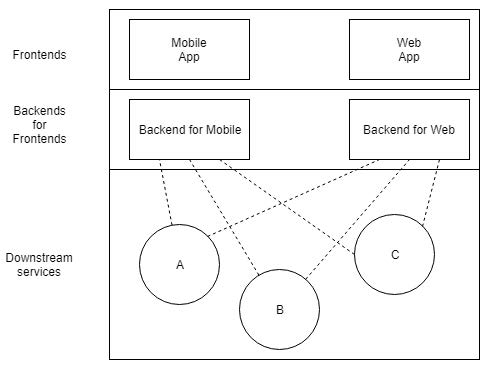
\includegraphics[width=0.9\textwidth]{content/1/chapter2/images/5.jpg}\\
图2.5 -面向前端的后端模式
\end{center}

使用\textbf{面向前端的后端(BFF)}的缺点是有些代码需要复制。只要这能够加速开发,并且从长期来看这只要不是一种负担,就没有问题,但需要密切关注在下游服务中聚合逻辑复制的可能性。有时,引入服务只是为了聚合类似的调用,可以帮助解决重复的问题。如果有多个前端,可以部分共享后端,而不会导致竞争。若正在为iOS和Android开发移动应用程序,可以考虑使用相同的后端,而为Web和/或桌面应用,则需要使用单独的后端。






















